%% Lines to compile only this capter
\[11pt, twoside, a4paper, openright]
\usepackage[utf8]{inputenc}
% \DeclareUnicodeCharacter{223C}{~}

%Bibliography style
% \usepackage[square, numbers]{natbib}
% \usepackage[round]{natbib}
% \usepackage{biblatex}
% \bibliographystyle{unsrtnat}
% \bibliographystyle{unsrt}
% \bibliographystyle{plain}
% \bibliographystyle{aa}
% \usepackage[backend=bibtex,style=authoryear,natbib=true]{biblatex} 
\usepackage[
backend=biber,
style=authoryear,
citestyle=authoryear,
url=false
]{biblatex}
\addbibresource{../source/library.bib}

\usepackage[T1]{fontenc}
\usepackage[french]{babel}
\usepackage{csquotes}  % used for citations (recommended when using biblatex)
%\usepackage{helvet}
%\renewcommand{\familydefault}{\sfdefault}
\usepackage{mathptmx}
\usepackage{amssymb}
\usepackage{geometry} 
\usepackage{xcolor}
\usepackage[absolute,overlay]{textpos}
\usepackage{graphicx}
\usepackage{lipsum}
\usepackage[explicit]{titlesec}
\usepackage{lmodern}
\usepackage{color}
\usepackage{array}
\usepackage{mathtools}
\usepackage{caption}
\usepackage{multicol}
\usepackage{booktabs}
\usepackage{enumitem}
\usepackage{hyperref}
\usepackage{afterpage}
\usepackage{emptypage}
\usepackage{setspace}
\usepackage{pgffor}
    \setlength{\columnseprule}{0pt}
    \setlength\columnsep{10pt}
\usepackage[francais,nohints]{minitoc}
    \setcounter{minitocdepth}{3}
 
 %https://la-bibliotex.fr/2019/02/03/ecrire-les-nombres-et-les-unites-avec-latex/   
\usepackage{siunitx}
% \sisetup{
%     detect-all,
%      output-decimal-marker={,},
%      group-minimum-digits = 3,
%      group-separator={~},
%      number-unit-separator={~},
%      inter-unit-product={~},
%      list-separator = {, },
%      list-final-separator = { et },
%      range-phrase = --,
%      separate-uncertainty = true,
%      multi-part-units = single,
%      list-units = single,
%      range-units = single
%     }
\usepackage{physics}
\usepackage{isotope}

\usepackage[perpage]{footmisc} % to reset the counter of footnote each page

    
\usepackage{fancyhdr}			% Entête et pieds de page. Doit être placé APRES geometry
\pagestyle{fancy}		% Indique que le style de la page sera justement fancy
%\lfoot[\thepage]{} 		% gauche du pied de page
%\cfoot{} 			% milieu du pied de page
%\rfoot[]{\thepage} 
\fancyfoot{} % vide le pied~de~page
\fancyfoot[LE,RO]{\thepage}
\fancyfoot[LO,CE]{}% droite du pied de page
\fancyhead{}	
\fancyhead[LE]{\leftmark}	
\fancyhead[RO]{\rightmark}

\fancypagestyle{plain}{%
\fancyhf{} % vide l’en-tête et le pied~de~page.
\fancyfoot[LE,RO]{\thepage} % numéro de la page en cours en gras% et centré en pied~de~page.
\renewcommand{\headrulewidth}{0pt}
\renewcommand{\footrulewidth}{0pt}}



% Premiere page des chapitres
\newlength\chapnumb
\setlength\chapnumb{3cm}
 
\titleformat{\chapter}[block] {
  \normalfont}{}{0pt} { %police
    \parbox[b]{\chapnumb}{
      \fontsize{120}{110}\selectfont\thechapter} %taille du chiffre
      \parbox[b]{\dimexpr\textwidth-\chapnumb\relax}{
        \raggedleft 
        \hfill{\bfseries\Huge#1}\\ %taille du titre
        \rule{\dimexpr\textwidth-\chapnumb\relax}{0.4pt} %ligne de separation
  }
}
 
 %premiere page chapitre non numerote (remerciement, table des matieres ...)
 
\titleformat{name=\chapter,numberless}[block]
{\normalfont}{}{0pt}
{   
    \parbox[b]{\dimexpr\textwidth}{%   
    \hfill{\bfseries\Huge#1}\\
  \rule{\dimexpr\textwidth}{0.4pt}}}
    
 %   \titleformat{name=\chapter,numberless}[block]
%{\normalfont}{}{0pt}
%{\parbox[b]{\chapnumb}{%
%   \mbox{}}%
%  \parbox[b]{\dimexpr\textwidth-\chapnumb\relax}{%
%    \raggedleft%
%    \hfill{\bfseries\Huge#1}\\
%    \rule{\dimexpr\textwidth-\chapnumb\relax}{0.4pt}}}


%%%    SIunitx
\sisetup{locale = FR,
  % inter-unit-product=\ensuremath{\cdot},
  inter-unit-product=\ensuremath{\,},
  per-mode=reciprocal,
  separate-uncertainty = true,
  detect-all
}
\DeclareSIUnit{\Mpc}{Mpc}
\DeclareSIUnit{\kpc}{kpc}
\DeclareSIUnit{\Gpc}{Gpc}
\DeclareSIUnit{\h}{\textit{h}~}
\DeclareSIUnit{\perh}{\textit{h}^{-1}\,}

%%% Geometry
\geometry{
left=20mm,
top=30mm,
right=20mm,
bottom=30mm
}

%%% Color
\definecolor{bordeau}{rgb}{0.3515625,0,0.234375}

%%% Commands
\newcommand{\Nmocks}{\num{30}}
\newcommand{\hMpc}{h^{-1}\,\mathrm{Mpc}}
\newcommand{\hGpc}{h^{-1}\,\mathrm{Gpc}}
\newcommand{\kms}{\mathrm{km\,s^{-1}}}

\newcommand{\lya}{Ly$\alpha$}
\newcommand{\lyb}{Ly$\beta$}
\newcommand{\lyalya}{Ly$\alpha$(Ly$\alpha$)}
\newcommand{\lyalyb}{Ly$\alpha$(Ly$\beta$)}

\newcommand{\lrf}{\lambda_{\rm RF}}
\newcommand{\kpar}{k_{\parallel}}
\newcommand{\apar}{\alpha_{\parallel}}
\newcommand{\rpar}{r_{\parallel}}
\newcommand{\aperp}{\alpha_{\perp}}
\newcommand{\rperp}{r_{\perp}}
\newcommand{\kperp}{k_{\perp}}

\newcommand{\blya}{b_{\rm Ly\alpha}}
\newcommand{\betalya}{\beta_{\rm Ly\alpha}}
\newcommand{\blyb}{b_{\rm Ly\alpha}}
\newcommand{\betalyb}{\beta_{\rm Ly\beta}}
\newcommand{\dlya}{d_{\rm Ly\alpha}}
\newcommand{\bhcd}{b_{\rm HCD}}
\newcommand{\betahcd}{\beta_{\rm HCD}}
\newcommand{\Fhcd}{F_{\rm HCD}}
\newcommand{\Lhcd}{L_{\rm HCD}}

\newcommand{\imin}{i_{\rm min}}
\newcommand{\imax}{i_{\rm max}}
\newcommand{\jmin}{j_{\rm min}}
\newcommand{\jmax}{j_{\rm max}}

\newcommand{\xioned}{\xi_{\rm 1d}}
\newcommand{\DHub}{D_{H}}
\newcommand{\DM}{D_{M}}

\newcommand{\omegam}{\Omega_M}
\newcommand{\omegac}{\Omega_C}
\newcommand{\omegab}{\Omega_B}
\newcommand{\omegan}{\Omega_\nu}
\newcommand{\omegal}{\Omega_\Lambda}
\newcommand{\omegak}{\Omega_k}
\newcommand{\orad}{\Omega_R}
\newcommand{\ogam}{\Omega_\gamma}
\newcommand{\lcdm}{$\Lambda$CDM}

\newcommand{\picca}{\texttt{picca}}

%%% Rem's command
\newcommand\blankpage{%
    \null
    \thispagestyle{empty}%
    \addtocounter{page}{-1}%
    \newpage}
  
% Command to set up a particular alignment for a cell in tabular :
% \myalign{c}{foo} for instance
\newcommand*{\myalign}[2]{\multicolumn{1}{#1}{#2}}
 
\renewcommand{\thesection}{\arabic{section}}

% Romain
\newcommand{\cRM}[1]{\MakeUppercase{\romannumeral #1}}	% Capital
\newcommand{\cRm}[1]{\textsc{\romannumeral #1}}	% Petit majuscule
\newcommand{\crm}[1]{\romannumeral #1}
% Siècle %
\newcommand{\siecle}[1]{\cRm{#1}\textsuperscript{e}~siècle}



% Thesis title
\newcommand{\PhDTitle}{Les forêts \lya{} du relevé eBOSS : comprendre les fonctions de corrélation et les systématiques} 

% Name
\newcommand{\PhDname}{Thomas Etourneau} 

% Change this variable if you add or remove chapters
\newcommand*{\NumOfChapters}{6}

% Change this variable if you add or remove appendices
\newcommand*{\NumOfAppendices}{2}

% PDF metadata
\hypersetup{
	pdfauthor={\PhDname},
	pdfsubject={Manuscrit de thèse de doctorat},
	pdftitle={\PhDTitle}
}


\begin{document}
%%

\graphicspath {{{{{{\figures/intro/}}}

\n-Chapter{\ to cosmology}
\minitoc
\newpage
\thisispagestyle{fancy}

The purpose of this first chapter is to introduce modern cosmology and briefly explain its construction over the last century. The idea is to give an overview of the current paradigm, while further detailing the key points needed for this manuscript. For an in-depth study of modern cosmology, we refer the reader to the following books:~\citet{Rich2010},~\citet{Dodelson2003}. 

\Section, "What Is Cosmology?
The term cosmogony (from the Greek \emph{cosmo-}: world; \emph{gon-}: to engender) refers to a conception and attempt to explain the birth of the world, and sometimes of man. There are a large number of cosmogonies, very often of religious origins. We can cite for example the Hindu cosmogony, in which the world is seen as a cycle: the god Brahma creates the world when he awakens, and destroys it when he falls asleep. Our universe thus corresponds to a day of Brahma, beginning when Brahma opens his eyes and ending when he closes them. The world thus follows a sequence of creation and destruction.
We can also quote the Abrahamic cosmogony, described in Genesis. This cosmogony is common to Judaism, Christianity, and Islam. In this cosmogony, the timeless creator god designed the world in 7 days. He began by creating light on the first day. He ended by creating Man in his own image on the sixth day, and then rested on the last day.
\begin{figure}
  \centering
  \includegraphics [scale=1]{cosmohindu.png}
  \Space.
  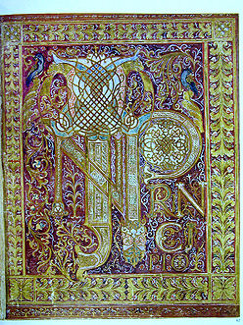
\includegraphics [scale=1]{genese.png}
  \nLeft: artistic illustration of Hindu cosmology. Right: cover of the book of Genesis, Bible of St. Paul Outside the Walls, circa 870.}
  \label...
\...end{figure}

We could spend the entire manuscript describing various cosmogonies. But the one we're interested in, and which we'll detail here, is the scientific cosmogony: \emph{cosmology}. Cosmology is therefore the study of the universe, its origin, its constituents and its future, within the framework of the scientific method. Even if today cosmology has a consensus among scientists regarding the understanding of the universe, this has not always been the case. For a long time, religious beliefs dominated, going so far as to limit or even prohibit scientific advances.
It wasn't until the 16th century that Copernicus proposed the heliocentric model, almost 2000 years after Aristotle's geocentric model, supported by the church and scientists until then.
% and thus opposes the geocentric model introduced by Aristotle and supported by the church and the scholars of the time.
Subsequently, Galileo's observations, Kepler's work and the emancipation of religious dogmas allowed the heliocentric model, based on Kepler's laws, to take hold. This also allowed Newton to propose his theory of gravitation shortly afterwards. This period marked the birth of physics and cosmology.

Until the \textsc{XIX} {\XIX} {\i~century, there was a consensus on the heliocentric model describing the universe as being limited to our solar system. Then emerged the idea that stars are other solar systems, notably thanks to the first distance measurements of nearby stars\for example the measurement of the distance of 61 Cygni by Bessel in 1838.}. The idea of galaxy, a system gathering a multitude of solar systems, is also emerging, leading us towards a less and less anthropocentric paradigm.

\paragraph{}
Modern cosmology was really born at the beginning of the century. In 1915, Einstein proposed his theory of gravitation: general relativity. It offers a radically different view from Newton's well-established theory. Gravitation is no longer seen as an instantaneous force between massive bodies but as a deformation of space-time propagating at the speed of light. Einstein's theory correctly predicts the advance of Mercury's perihelion, the value of which was previously misunderstood. Then in 1919 during an eclipse of the Sun, the deviation of light by a massive body, a direct prediction of general relativity and not present in Newton's theory, is observed. Not only was the deviation of light observed for the first time, but the angle of deviation observed corresponded to that predicted by the theory. This establishes Einstein's theory as a new theory of gravitation within the scientific community.

Furthermore, observational cosmology is making remarkable progress, notably thanks to the

Translated with www.DeepL.com/Translator (free version)